% Options for packages loaded elsewhere
\PassOptionsToPackage{unicode}{hyperref}
\PassOptionsToPackage{hyphens}{url}
%
\documentclass[
  man]{apa7}
\usepackage{amsmath,amssymb}
\usepackage{iftex}
\ifPDFTeX
  \usepackage[T1]{fontenc}
  \usepackage[utf8]{inputenc}
  \usepackage{textcomp} % provide euro and other symbols
\else % if luatex or xetex
  \usepackage{unicode-math} % this also loads fontspec
  \defaultfontfeatures{Scale=MatchLowercase}
  \defaultfontfeatures[\rmfamily]{Ligatures=TeX,Scale=1}
\fi
\usepackage{lmodern}
\ifPDFTeX\else
  % xetex/luatex font selection
\fi
% Use upquote if available, for straight quotes in verbatim environments
\IfFileExists{upquote.sty}{\usepackage{upquote}}{}
\IfFileExists{microtype.sty}{% use microtype if available
  \usepackage[]{microtype}
  \UseMicrotypeSet[protrusion]{basicmath} % disable protrusion for tt fonts
}{}
\makeatletter
\@ifundefined{KOMAClassName}{% if non-KOMA class
  \IfFileExists{parskip.sty}{%
    \usepackage{parskip}
  }{% else
    \setlength{\parindent}{0pt}
    \setlength{\parskip}{6pt plus 2pt minus 1pt}}
}{% if KOMA class
  \KOMAoptions{parskip=half}}
\makeatother
\usepackage{xcolor}
\usepackage{graphicx}
\makeatletter
\def\maxwidth{\ifdim\Gin@nat@width>\linewidth\linewidth\else\Gin@nat@width\fi}
\def\maxheight{\ifdim\Gin@nat@height>\textheight\textheight\else\Gin@nat@height\fi}
\makeatother
% Scale images if necessary, so that they will not overflow the page
% margins by default, and it is still possible to overwrite the defaults
% using explicit options in \includegraphics[width, height, ...]{}
\setkeys{Gin}{width=\maxwidth,height=\maxheight,keepaspectratio}
% Set default figure placement to htbp
\makeatletter
\def\fps@figure{htbp}
\makeatother
\setlength{\emergencystretch}{3em} % prevent overfull lines
\providecommand{\tightlist}{%
  \setlength{\itemsep}{0pt}\setlength{\parskip}{0pt}}
\setcounter{secnumdepth}{-\maxdimen} % remove section numbering
% Make \paragraph and \subparagraph free-standing
\ifx\paragraph\undefined\else
  \let\oldparagraph\paragraph
  \renewcommand{\paragraph}[1]{\oldparagraph{#1}\mbox{}}
\fi
\ifx\subparagraph\undefined\else
  \let\oldsubparagraph\subparagraph
  \renewcommand{\subparagraph}[1]{\oldsubparagraph{#1}\mbox{}}
\fi
\newlength{\cslhangindent}
\setlength{\cslhangindent}{1.5em}
\newlength{\csllabelwidth}
\setlength{\csllabelwidth}{3em}
\newlength{\cslentryspacingunit} % times entry-spacing
\setlength{\cslentryspacingunit}{\parskip}
\newenvironment{CSLReferences}[2] % #1 hanging-ident, #2 entry spacing
 {% don't indent paragraphs
  \setlength{\parindent}{0pt}
  % turn on hanging indent if param 1 is 1
  \ifodd #1
  \let\oldpar\par
  \def\par{\hangindent=\cslhangindent\oldpar}
  \fi
  % set entry spacing
  \setlength{\parskip}{#2\cslentryspacingunit}
 }%
 {}
\usepackage{calc}
\newcommand{\CSLBlock}[1]{#1\hfill\break}
\newcommand{\CSLLeftMargin}[1]{\parbox[t]{\csllabelwidth}{#1}}
\newcommand{\CSLRightInline}[1]{\parbox[t]{\linewidth - \csllabelwidth}{#1}\break}
\newcommand{\CSLIndent}[1]{\hspace{\cslhangindent}#1}
\ifLuaTeX
\usepackage[bidi=basic]{babel}
\else
\usepackage[bidi=default]{babel}
\fi
\babelprovide[main,import]{english}
% get rid of language-specific shorthands (see #6817):
\let\LanguageShortHands\languageshorthands
\def\languageshorthands#1{}
% Manuscript styling
\usepackage{upgreek}
\captionsetup{font=singlespacing,justification=justified}

% Table formatting
\usepackage{longtable}
\usepackage{lscape}
% \usepackage[counterclockwise]{rotating}   % Landscape page setup for large tables
\usepackage{multirow}		% Table styling
\usepackage{tabularx}		% Control Column width
\usepackage[flushleft]{threeparttable}	% Allows for three part tables with a specified notes section
\usepackage{threeparttablex}            % Lets threeparttable work with longtable

% Create new environments so endfloat can handle them
% \newenvironment{ltable}
%   {\begin{landscape}\centering\begin{threeparttable}}
%   {\end{threeparttable}\end{landscape}}
\newenvironment{lltable}{\begin{landscape}\centering\begin{ThreePartTable}}{\end{ThreePartTable}\end{landscape}}

% Enables adjusting longtable caption width to table width
% Solution found at http://golatex.de/longtable-mit-caption-so-breit-wie-die-tabelle-t15767.html
\makeatletter
\newcommand\LastLTentrywidth{1em}
\newlength\longtablewidth
\setlength{\longtablewidth}{1in}
\newcommand{\getlongtablewidth}{\begingroup \ifcsname LT@\roman{LT@tables}\endcsname \global\longtablewidth=0pt \renewcommand{\LT@entry}[2]{\global\advance\longtablewidth by ##2\relax\gdef\LastLTentrywidth{##2}}\@nameuse{LT@\roman{LT@tables}} \fi \endgroup}

% \setlength{\parindent}{0.5in}
% \setlength{\parskip}{0pt plus 0pt minus 0pt}

% Overwrite redefinition of paragraph and subparagraph by the default LaTeX template
% See https://github.com/crsh/papaja/issues/292
\makeatletter
\renewcommand{\paragraph}{\@startsection{paragraph}{4}{\parindent}%
  {0\baselineskip \@plus 0.2ex \@minus 0.2ex}%
  {-1em}%
  {\normalfont\normalsize\bfseries\itshape\typesectitle}}

\renewcommand{\subparagraph}[1]{\@startsection{subparagraph}{5}{1em}%
  {0\baselineskip \@plus 0.2ex \@minus 0.2ex}%
  {-\z@\relax}%
  {\normalfont\normalsize\itshape\hspace{\parindent}{#1}\textit{\addperi}}{\relax}}
\makeatother

\makeatletter
\usepackage{etoolbox}
\patchcmd{\maketitle}
  {\section{\normalfont\normalsize\abstractname}}
  {\section*{\normalfont\normalsize\abstractname}}
  {}{\typeout{Failed to patch abstract.}}
\patchcmd{\maketitle}
  {\section{\protect\normalfont{\@title}}}
  {\section*{\protect\normalfont{\@title}}}
  {}{\typeout{Failed to patch title.}}
\makeatother

\usepackage{xpatch}
\makeatletter
\xapptocmd\appendix
  {\xapptocmd\section
    {\addcontentsline{toc}{section}{\appendixname\ifoneappendix\else~\theappendix\fi\\: #1}}
    {}{\InnerPatchFailed}%
  }
{}{\PatchFailed}
\keywords{Measurement Invariance\newline\indent Word count: X}
\DeclareDelayedFloatFlavor{ThreePartTable}{table}
\DeclareDelayedFloatFlavor{lltable}{table}
\DeclareDelayedFloatFlavor*{longtable}{table}
\makeatletter
\renewcommand{\efloat@iwrite}[1]{\immediate\expandafter\protected@write\csname efloat@post#1\endcsname{}}
\makeatother
\usepackage{csquotes}
\ifLuaTeX
  \usepackage{selnolig}  % disable illegal ligatures
\fi
\IfFileExists{bookmark.sty}{\usepackage{bookmark}}{\usepackage{hyperref}}
\IfFileExists{xurl.sty}{\usepackage{xurl}}{} % add URL line breaks if available
\urlstyle{same}
\hypersetup{
  pdftitle={Bought but Paritially Sold? Measurement Invariance across Purchased and Snowball Samples},
  pdfauthor={John Kulas1, Casey Osorio-Duffoo3, Mike Defabiis2, \& Morgan Russell2},
  pdflang={en-EN},
  pdfkeywords={Measurement Invariance},
  hidelinks,
  pdfcreator={LaTeX via pandoc}}

\title{Bought but Paritially Sold? Measurement Invariance across Purchased and Snowball Samples}
\author{John Kulas\textsuperscript{1}, Casey Osorio-Duffoo\textsuperscript{3}, Mike Defabiis\textsuperscript{2}, \& Morgan Russell\textsuperscript{2}}
\date{}


\shorttitle{Measurement Invariance}

\authornote{

Add complete departmental affiliations for each author here. Each new line herein must be indented, like this line.

Enter author note here.

Correspondence concerning this article should be addressed to John Kulas, 1 Awesome Lane, Mosquitosota. E-mail: \href{mailto:jtkulas@ergreports.com}{\nolinkurl{jtkulas@ergreports.com}}

}

\affiliation{\vspace{0.5cm}\textsuperscript{1} eRg\\\textsuperscript{2} Harver\\\textsuperscript{3} Montclair State University}

\abstract{%
The literature tilts predominantly positive regarding the benefits of ``purchased'' samples that have become more prevalent within organizational surveying applications within the past 15 or so years. The current study first explores the measurement invariance of an 18-item engagement survey across three different samples before conducting a follow-up across five: 1) voluntary snowball, 2) cleaned Qualtrics, 3) cleaned Prolific, 4) flagged Qualtrics, and 5) flagged Prolific.
}



\begin{document}
\maketitle

First emerging in the 1990's (Li et al., 1999), commercial online panel data (OPD) is more commonly encountered, although questions regarding data quality persist {[}Walter et al. (2019); {]}. Walter et al. (2019) did a meta-analysis

Porter et al. (2019)'s qualitative review concluded with practical recomendations such as

The appeal is obvious - other than the financial obstacle, these OPD options bypass the so-called ``courtship rituals'' that are often (at least percieved to be) necessary when attempting to sample from organizational populations (e.g., Tracy, 2019)

Need help finding:

\begin{itemize}
\tightlist
\item
  Walter et al. (2019)
\end{itemize}

The roots of employee {[}aka work; e.g., W. Schaufeli and Bakker (2010){]} engagement research likely started with theoretical expansions of forms of employee participation (see, for example, Ferris \& Hellier, 1984) and job involvement (e.g., Elloy et al., 1991). This exploration extended into broader considerations of attitudes and emotions (Staw et al., 1994) and were informed by further exploration of the dimensionality of constructs such as organizational commitment (Meyer \& Allen, 1991). The 1990's saw focused development and refinement (for example, a dissertation; Leone (1995) or actual semantic reference; Kahn (1990a)). Staw et al. (1994) investigated the relationships between \emph{positive emotions} and favorable work outcomes, and although they do not use the word, ``engagement'', their distinction between felt and expressed emotion likely held influence upon the burgeoning interest in the engagement construct.

Clear in this history is the specification of engagement as a work \emph{attitude}.

Although occasionally referred to as residing on the opposing pole to \emph{burnout} (Maslach \& Leiter, 2008), these two constructs are currently most commonly conceptualized as being distinct (Goering et al., 2017; Kim et al., 2009; Schaufeli et al., 2008; Timms et al., 2012), although certainly not universally (Cole et al., 2012; Taris et al., 2017). Comparing the two, Goering et al. (2017) concluded that they have a moderate (negative) association, but also distinct nomological networks. Schaufeli et al. (2008) investigated both internal and external association indicators, concluding that engagement and burnout (as well as \emph{workaholism}) should be considered three distinct constructs.

Burnout can be defined as a psychological syndrome characterized by exhaustion (low energy), cynicism (low involvement), and inefficacy (low self-efficacy), which is experienced in response to chronic job stressors (e.g., Leiter \& Maslach, 2004; Maslach \& Leiter, 1997). Alternatively, engagement refers to an individual worker's involvement and satisfaction as well as enthusiasm for work (Harter et al., 2002). Schaufeli and Bakker (2003) further specify a ``positive, fulfilling, work-related state of mind that is characterized by vigor, dedication, and absorption'' (p.~74). Via their conceptualization, vigor is described as high levels of energy and mental resilience while working. Dedication refers to being strongly involved in one's work and experiencing a sense of significance, enthusiasm, inspiration, pride, and challenge. Absorption is characterized by being fully concentrated and happily engrossed in one's work, whereby time passes quickly and one has difficulties with detaching oneself from work (Schaufeli et al., 2002). The dimension of absorption has been noted as being influenced in conceptual specification by (Csikszentmihalyi, 1990)'s concept of ``flow''.

Regarding measurement, Gallup is widely acknowledged as an early pioneer in the measurement of the construct (see, for example, Coffman \& Harter, 1999). The Utrecht Work Engagement Scale (UWES) is another self-report questionnaire developed by Schaufeli and Bakker (2003) that directly assesses the vigor, dedication, and absorption elements.

\hypertarget{attitudes}{%
\subsection{Attitudes}\label{attitudes}}

\begin{quote}
TRIPARTITE MODEL--work here
\end{quote}

The first, to our knowledge, use of the word ``engagement'' as a construct came in Kahn (1990b), defining it as: ``the harnessing of organization members' selves to their work roles; in engagement, people employ and express themselves physically, cognitively, and emotionally during role performances.'' Although this definition was quickly bypassed by subsequent papers (see, for example, (Baumruk, 2004) and (Shaw, 2005), who framed it in terms of one's cognitive and affective \emph{commitment} to one's organization), Kahn (1990b)'s definition is notable in that it conforms to the then-ascendant tripartite model of attitudes proposed by Rosenberg (1960). This model frames attitudes as latent variables that manifest cognitively, affectively and behaviorally.

Although falling out of favor in the decades following its construction, interest in the tripartite model was revived by Kaiser and Wilson (2019),

\hypertarget{item-order-as-a-multidimensional-assessment-response-cues}{%
\subsection{Item order as a multidimensional assessment response cues}\label{item-order-as-a-multidimensional-assessment-response-cues}}

Response cues in general and order effects in particular have their root in Cognitive Psychology, with the bulk of studies occurring in the early days of Cognitive Psychology (e.g., the 1960's on). Primacy and recency (whether an item is presented at the beginning or end of a list) are known to elicit differences in response (e.g., \textbf{krosnick1987evaluation?}). This effect has also been noted in methodological contexts in the form of differential carryover effects. For example, the order of presentation of samples in a product taste test (see, for example, \textbf{dean1980presentation?}). (\textbf{ackerman1989comparison?}) found only small differences in response patterns when presenting \emph{test} items in a fixed versus random ordering. (\textbf{mashburn2014effect?}) experimentally controlled the presentation of rated material, finding higher indices of reliability and validity of ratings when content was administered randomly (e.g., order effects were controlled for).

(\textbf{knowles1988item?}) and (\textbf{hamilton1990self?}) both administered exhaustively crossed orderings of items, noting better item discrimination (e.g., corrected item-total correlations) \emph{later} in the assessment, regardless of actual item content. (\textbf{steinberg1994context?}) provides a description of this effect: ``\ldots literature converges on the view that responding repeatedly to items representing a single, unidimensional psychological construct increases the accessibility of relevant beliefs or feelings, which in turn, increases the relation between the item resopnse and the underlying construct.'' (p.~341) This statement could be rephrased as: location serves as a response cue. ``This attentional focus influences item responses through such processes as item interpretation and ease of retrieval of relevant feelings that are applied to the item'' (\textbf{steinberg1994context?}).

(\textbf{steinberg1994context?}) looked at order effects in personality measurement,

\begin{quote}
Weinberg, M. K., Seton, C., \& Cameron, N. (2018). The Measurement of Subjective Wellbeing: Item-Order Effects in the Personal Wellbeing Index---Adult. Journal of Happiness Studies, 19(1), 315--332. \url{https://doi-org.ezproxy.montclair.edu/10.1007/s10902-016-9822-1}
\end{quote}

(\textbf{Weinberg2018?}) examine the effects of randomized items and domains in the Personal Wellbeing Index (PWI) in measure subjective wellbeing (SWB). (\textbf{Weinberg2018?}) conduct two studies one, looking at the PWI comparing its usual general-specific format to a modified format, furthermore, the order of the domain items will stay the same, while the general items will be random in question order. In the second study, (\textbf{Weinberg2018?}) randomized the domain items while the general items will be the same to standard scale order. In (\textbf{Weinberg2018?}), study 1 showed no results between general specific format and the modified format, however in study 2, they did find that presenting the random order effects did have lower means, then fixed order effects. (\textbf{Weinberg2018?}) present many different reasons for this outcomes, which could be those in the random order effect group had more participant experiencing high levels of wellbeing, and the other explanation is that changing order of items of PWI could affect the score. (\textbf{Weinberg2018?}) conducted a multiple regression analysis which showed that random order group account for 9\% more variance in GLS than the fixed order group and conducted a confirmatory factor analysis showing that the fixed order groups was not a good model fit.

(\textbf{serico2021?}) looked at item order effects in self-report measures of aggression perpetration and victimization. (\textbf{serico2021?}) provides a descriptions of two general biases in self-report measures, which are the subject's biases, and bias in wording, order, or format of items in the measure. In previous studies, there was an item order effect and item group effect in the measure that shows participants' response and psychometric properties of an aggression measure. \# citation from other articles (Dietz \& Jasinski, 2007; Shorey, Woods, \& Cornelius, 2016). \#\#\#\#\#\#\#\#\# In (\textbf{serico2021?}), the findings shows that there is an item order affect in the reported frequency of aggression perpetration. It shows that item order can influence a person self-report in aggression perpetration and victimization, showing that there are methodological issue that have to be consider when developing and utilizing measure of aggression and victimization. This methodological issues can still be applicable to other measure such as workplace engagement, since we also look at people's behaviors, cognitive, and emotions.

This model is not without criticism, however. Some critics question its structural validity by pointing out that vigor, dedication and absorption all correlate highly with each other (Kulikowski, 2017).

The present article explores two methods for constructing a scale that incorporates both the substantive and attitudinal models into one, a more classical one based on corrected item-total correlations and one based on modification indices.

Existing measures include (\textbf{soane2012development?})

Our conceptualization of work engagement is a mental state wherein employees: a) feel energized (\emph{Vigor}), b) are enthusiastic about the content of their work and the things they do (\emph{Dedication}), and c) are so immersed in their work activities that time seems compressed (\emph{Absorption}). We further decompose each of these facets into three attitudinal components: d) feeling (e.g., affect), e) thought (e.g., cognition), and f) action (e.g., behavior). Development and construct validation of the focal 18-item measure of engagement is described in Russell et al. (2022) whereas the current study on administrative response cues in the form of order of item presentation. The expectation is that either model (attitudinal or substantive) will exhibit stronger factorial validity when item administration parallels latent structure.

\hypertarget{panels}{%
\subsection{Panels}\label{panels}}

Landers and Behrend (2015) encourage researchers to avoid broad classifications such as good and bad regarding samples and sampling methodologies, concluding that online panels may be qualitatively ``different'' from traditional convenience samples, but they should not be stigmatized simply because they're different. Cheung et al. (2017) conducted a thorough review of one of the earliest platforms to emerge within the realm of organziational research, MTurk, and highlighted a number of noted limitations, but provided redcommendations for addressing each limitation while again cautioning against negative stereotypes. Walter et al. (2019) performed a meta-analysis focused on internal consistency estimates as well as IV-DV effects, noting similar results stemming from online panels (when compared to more traditional data sources).

\hypertarget{methods}{%
\section{Methods}\label{methods}}

\hypertarget{participants}{%
\subsection{Participants}\label{participants}}

Data was obtained from three sources. In the first sampling, 743 individuals responded to a Qualtrics panel survey including the focal survey as well as 2 convergent validation measures, 2 discriminant validation measures, and one criterion measure (good/bad pretty even 366 vs 377). The second sampling was identical to the first in survey composition, but the respondents were snowball sampled, initiated from the authors and colleagues (n = 232). The third data source was a Prolific sample (\emph{n}=785), and the survey battery differed in content (currently good = 568, bad = 96; probably need harsher screen or also include NAs).

\hypertarget{materials}{%
\subsection{Materials}\label{materials}}

Our 18-item engagement measure was crafted to be intentionally complex (each item is intended to load on two constructs). This complexity, however, derives from a crossing of the attitudinal components of affect, cognition, and behavior with the substantive engagement components of vigor, dedication, and absorption. Within the current investigation, we realized \(\alpha\)'s of (Absorption), (Dedication), (Vigor), (Affect), (Cognition), and (Behavior). The 6-point response scale is: Strongly Disagree, Disagree, Somewhat Disagree, Somewhat Agree, Agree, Strongly Agree. The item stems as well as their scale associations are presented in Table XX.

\hypertarget{analysis}{%
\subsection{Analysis}\label{analysis}}

three datasets:

\begin{itemize}
\tightlist
\item
  Engagement+(Attitudinal/Substantive) Qualtrics (n=743)
\item
  initial\_data\_screen/inprogress Prolific (n=784)
\item
  Engagement(post-Qualtrics) Snowball (n=232)
\end{itemize}

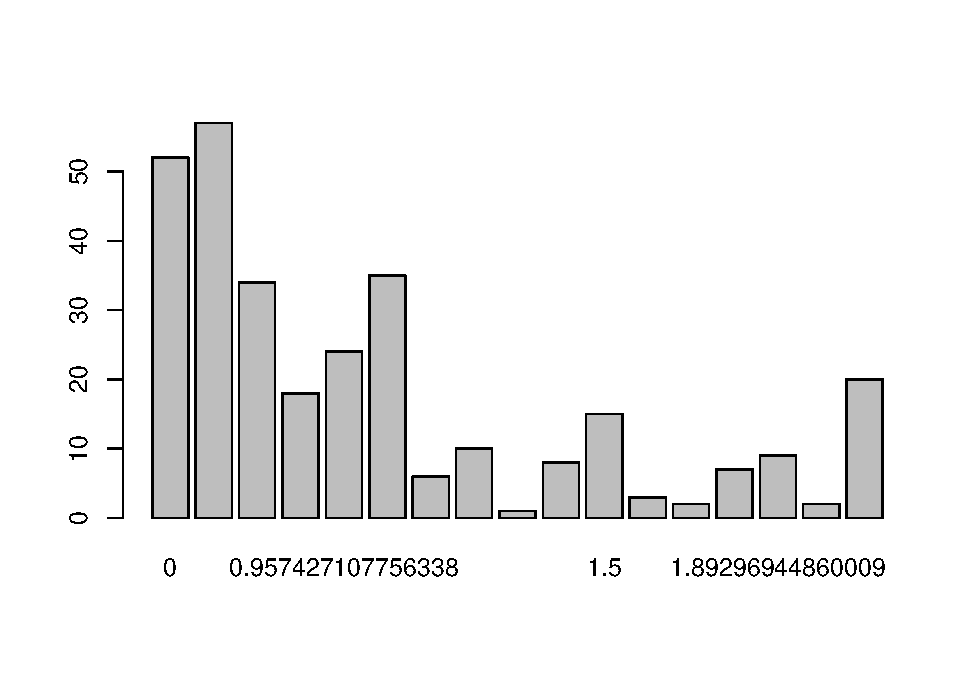
\includegraphics{Measurement_Invariance_files/figure-latex/unnamed-chunk-1-1.pdf}

\begin{verbatim}
## newdata.att$irv2 
##                   Frequency  Percent Valid Percent
## 0                        52  15.2493       17.1617
## 0.5                      57  16.7155       18.8119
## 0.577350269189626        34   9.9707       11.2211
## 0.816496580927726        18   5.2786        5.9406
## 0.957427107756338        24   7.0381        7.9208
## 1                        35  10.2639       11.5512
## 1.15470053837925          6   1.7595        1.9802
## 1.25830573921179         10   2.9326        3.3003
## 1.29099444873581          1   0.2933        0.3300
## 1.4142135623731           8   2.3460        2.6403
## 1.5                      15   4.3988        4.9505
## 1.63299316185545          3   0.8798        0.9901
## 1.70782512765993          2   0.5865        0.6601
## 1.73205080756888          7   2.0528        2.3102
## 1.89296944860009          9   2.6393        2.9703
## 1.91485421551268          2   0.5865        0.6601
## 2                        20   5.8651        6.6007
## NA's                     38  11.1437              
## Total                   341 100.0000      100.0000
\end{verbatim}

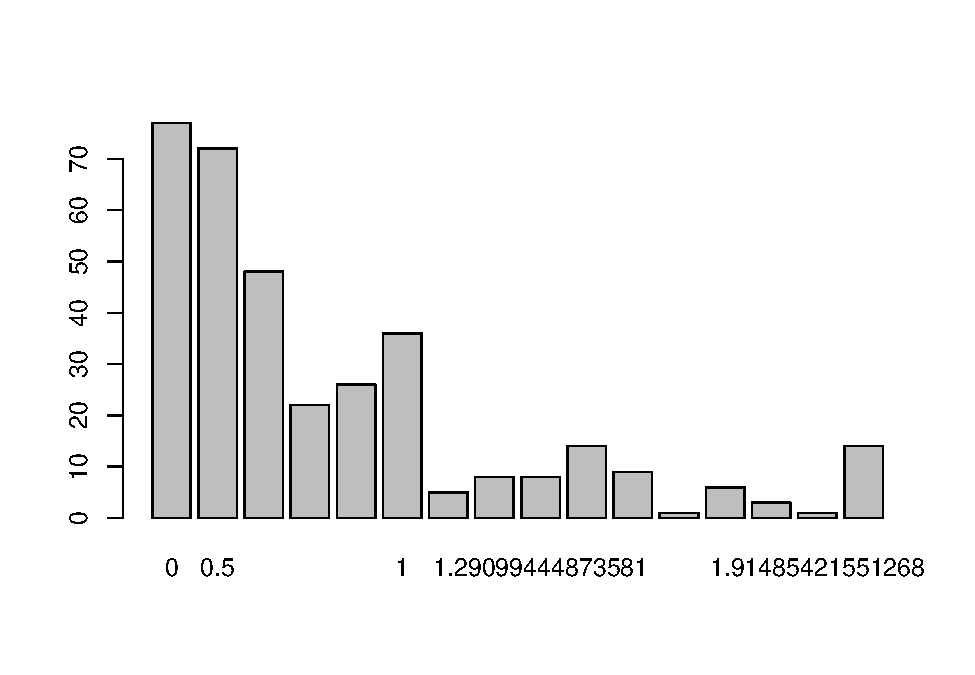
\includegraphics{Measurement_Invariance_files/figure-latex/unnamed-chunk-1-2.pdf}

\begin{verbatim}
## newdata.sub$irv2 
##                   Frequency  Percent Valid Percent
## 0                        77  19.1542       22.0000
## 0.5                      72  17.9104       20.5714
## 0.577350269189626        48  11.9403       13.7143
## 0.816496580927726        22   5.4726        6.2857
## 0.957427107756338        26   6.4677        7.4286
## 1                        36   8.9552       10.2857
## 1.15470053837925          5   1.2438        1.4286
## 1.25830573921179          8   1.9900        2.2857
## 1.29099444873581          8   1.9900        2.2857
## 1.4142135623731          14   3.4826        4.0000
## 1.5                       9   2.2388        2.5714
## 1.70782512765993          1   0.2488        0.2857
## 1.73205080756888          6   1.4925        1.7143
## 1.89296944860009          3   0.7463        0.8571
## 1.91485421551268          1   0.2488        0.2857
## 2                        14   3.4826        4.0000
## NA's                     52  12.9353              
## Total                   402 100.0000      100.0000
\end{verbatim}

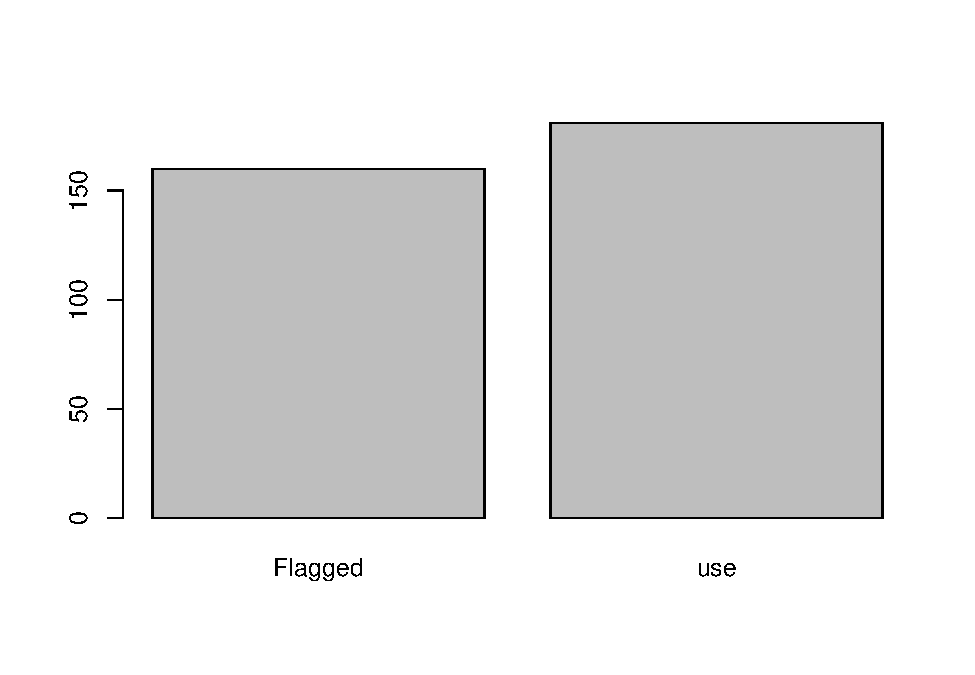
\includegraphics{Measurement_Invariance_files/figure-latex/unnamed-chunk-1-3.pdf}

\begin{verbatim}
## newdata.att$flag 
##         Frequency Percent
## Flagged       160   46.92
## use           181   53.08
## Total         341  100.00
\end{verbatim}

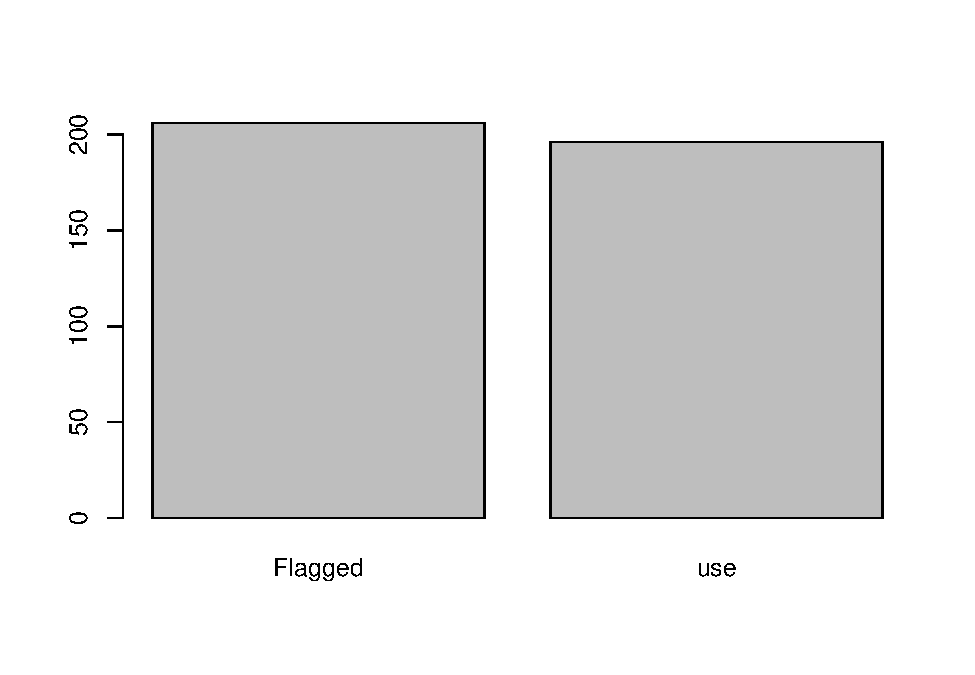
\includegraphics{Measurement_Invariance_files/figure-latex/unnamed-chunk-1-4.pdf}

\begin{verbatim}
## newdata.sub$flag 
##         Frequency Percent
## Flagged       206   51.24
## use           196   48.76
## Total         402  100.00
\end{verbatim}

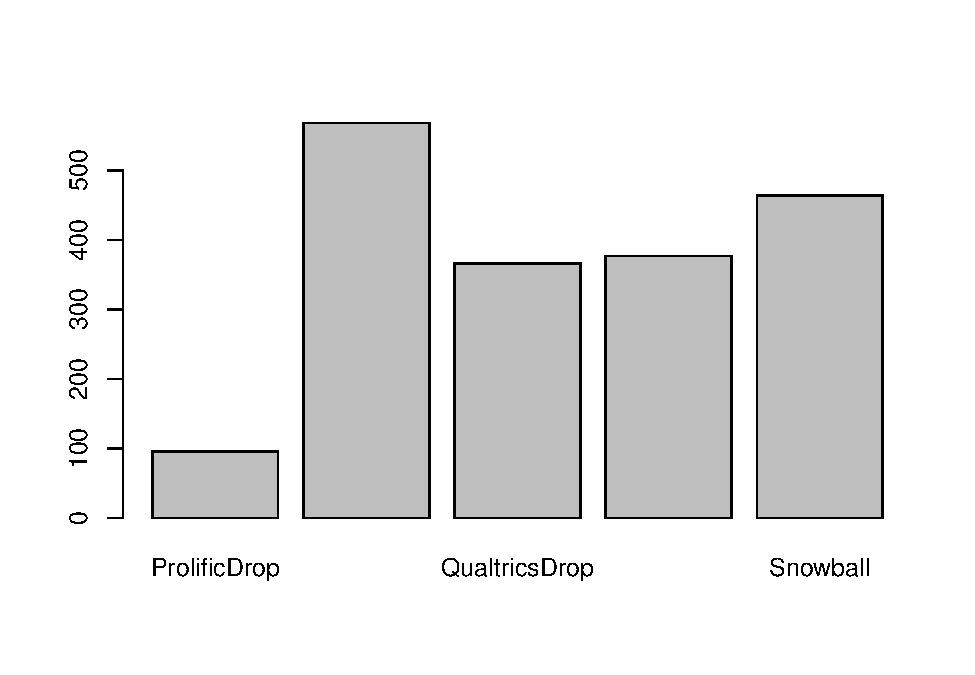
\includegraphics{Measurement_Invariance_files/figure-latex/unnamed-chunk-1-5.pdf}

\begin{verbatim}
## analyses$from 
##               Frequency Percent
## ProlificDrop         96   5.131
## ProlificKeep        568  30.358
## QualtricsDrop       366  19.562
## QualtricsKeep       377  20.150
## Snowball            464  24.800
## Total              1871 100.000
\end{verbatim}

\hypertarget{results}{%
\section{Results}\label{results}}

We used R {[}Version 4.3.1; R Core Team (2021){]} for all our analyses.

\begin{verbatim}
##     
##      ProlificDrop ProlificKeep QualtricsDrop QualtricsKeep Snowball
##   0             8          561           310           333      232
##   1             0            7             0             0        0
##   21           88            0            56            44      232
\end{verbatim}

The omnibus CFA's, regardless of item ordering, across respondents showed fair fit for both the substantive (\(\chi^2_{substantive}\)=, \emph{df}=, \emph{RMSEA}=) as well as attitudinal structures (\(\chi^2_{attitudinal}\)=, \emph{df}=, \emph{RMSEA}=). Additional fit indices for the two models are presented in Table XX. Figures 1 and 2 present the omnibus models visually (standardized coefficients displayed). Note that the primary source of misfit for both models within the omnibus analysis is item 14, which is the lone reverse-coded item within the inventory, ``Thinking about work saps my energy''.

\hypertarget{condition-effects}{%
\subsubsection{Condition effects}\label{condition-effects}}

The order of item presentation was: 1) random within substantive dimension, 2) random within attitudinal dimension, 3) parcels of substantive within attitudinal (36-item attitudinal context), 4) parcels of attitudinal within substantive (36-item substantive context), 5) parcels of substantive within attitudinal (20-item attitudinal context), and 6) parcels of attitudinal within substantive (20-item substantive context). For example, in condition 1, the first items presented were all associated with one attitudinal dimension (for example, ``Affect''). Once the Affect item list was fully exhausted, the respondent was then administered the full set of Behavioral items, and once these were completed the respondent was then administered the Cognitive item set\footnote{Across conditions, the order of presentation of item ``blocks'' was also randomized. For example, not all respondents in Condition 1 was administered the Affect item block first - roughly 1/3 was presented the Behavioral block first and roughly 1/3 was presented the Cognitive block first.}. We view these orderings as cues regarding factor structure, and anticipated empirical factor structures to reflect these cues. The effects did emerge, but were quite moderate (for example, \(\Delta{\chi^2_{Cond1}}\) = 9.55, \(\Delta{AIC_{Cond1}}\) = 10.53). Given the variety of item orderings administered, this should be considered somewhat comforting regarding the effect of contextual embeddedness within multidimensional inventories. To further explore degree of similarity, we applied explicit tests of measurement invariance.

\hypertarget{measurement-invariance}{%
\paragraph{Measurement invariance}\label{measurement-invariance}}

Because our six conditions were obtained across two different sampling procedures, we apply our analyses of measurement invariance twice - first investigating the four conditions administered within our initial snowball sampling and then secondly also extending to the follow-up Qualtrics panel respondents.

We looked at structural invariance as well as latent means (Meredith, 1993; Steinmetz et al., 2009).

\hypertarget{discussion}{%
\section{Discussion}\label{discussion}}

The item cues did provide slight response cues (attending to individual model fit indices), however, the effect was quite small. Measurement invariance is plausible within our initial four administration conditions, although it is not attained across all six conditions. This is possibly attributable to differences in sampled population (in addition to the possibility that this difference is attributable to item orderings),

\newpage

\hypertarget{references}{%
\section{References}\label{references}}

\begingroup
\setlength{\parindent}{-0.5in}
\setlength{\leftskip}{0.5in}

\hypertarget{refs}{}
\begin{CSLReferences}{1}{0}
\leavevmode\vadjust pre{\hypertarget{ref-baumruk2004missing}{}}%
Baumruk, R. (2004). \emph{The missing link: The role of employee engagement in business success}. \emph{47}, 48--52.

\leavevmode\vadjust pre{\hypertarget{ref-cheung2017amazon}{}}%
Cheung, J. H., Burns, D. K., Sinclair, R. R., \& Sliter, M. (2017). Amazon mechanical turk in organizational psychology: An evaluation and practical recommendations. \emph{Journal of Business and Psychology}, \emph{32}, 347--361.

\leavevmode\vadjust pre{\hypertarget{ref-coffman_hard_1999}{}}%
Coffman, C., \& Harter, J. (1999). A hard look at soft numbers. \emph{Position Paper, Gallup Organization}.

\leavevmode\vadjust pre{\hypertarget{ref-cole2012job}{}}%
Cole, M. S., Walter, F., Bedeian, A. G., \& O'Boyle, E. H. (2012). Job burnout and employee engagement: A meta-analytic examination of construct proliferation. \emph{Journal of Management}, \emph{38}(5), 1550--1581.

\leavevmode\vadjust pre{\hypertarget{ref-csikszentmihalyi1990flow}{}}%
Csikszentmihalyi, M. (1990). \emph{Flow: The psychology of optimal experience} (Vol. 1990). Harper \& Row New York.

\leavevmode\vadjust pre{\hypertarget{ref-elloy_examination_1991}{}}%
Elloy, D. F., Everett, J. E., \& Flynn, W. R. (1991). An examination of the correlates of job involvement. \emph{Group \& Organization Studies}, \emph{16}(2), 160--177. \url{https://doi.org/10.1177/105960119101600204}

\leavevmode\vadjust pre{\hypertarget{ref-ferris_added_1984}{}}%
Ferris, R., \& Hellier, P. (1984). Added value productivity schemes and employee participation. \emph{Asia Pacific Journal of Human Resources}, \emph{22}(4), 35--44. \url{https://doi.org/10.1177/103841118402200406}

\leavevmode\vadjust pre{\hypertarget{ref-goering2017not}{}}%
Goering, D. D., Shimazu, A., Zhou, F., Wada, T., \& Sakai, R. (2017). Not if, but how they differ: A meta-analytic test of the nomological networks of burnout and engagement. \emph{Burnout Research}, \emph{5}, 21--34.

\leavevmode\vadjust pre{\hypertarget{ref-harter_business-unit-level_2002}{}}%
Harter, J. K., Schmidt, F. L., \& Hayes, T. L. (2002). Business-unit-level relationship between employee satisfaction, employee engagement, and business outcomes: A meta-analysis. \emph{Journal of Applied Psychology}, \emph{87}(2), 268.

\leavevmode\vadjust pre{\hypertarget{ref-kahn1990psychological}{}}%
Kahn, W. A. (1990b). Psychological conditions of personal engagement and disengagement at work. \emph{Academy of Management Journal}, \emph{33}(4), 692--724.

\leavevmode\vadjust pre{\hypertarget{ref-kahn_psychological_1990}{}}%
Kahn, W. A. (1990a). Psychological conditions of personal engagement and disengagement at work. \emph{Academy of Management Journal}, \emph{33}(4), 692--724.

\leavevmode\vadjust pre{\hypertarget{ref-kaiser_campbell_2019}{}}%
Kaiser, F. G., \& Wilson, M. (2019). The {Campbell} {Paradigm} as a {Behavior}-{Predictive} {Reinterpretation} of the {Classical} {Tripartite} {Model} of {Attitudes}. \emph{European Psychologist}, \emph{24}(4), 359--374. \url{https://doi.org/10.1027/1016-9040/a000364}

\leavevmode\vadjust pre{\hypertarget{ref-kim_burnout_2009}{}}%
Kim, H. J., Shin, K. H., \& Swanger, N. (2009). Burnout and engagement: {A} comparative analysis using the {Big} {Five} personality dimensions. \emph{International Journal of Hospitality Management}, \emph{28}(1), 96--104. \url{https://doi.org/10.1016/j.ijhm.2008.06.001}

\leavevmode\vadjust pre{\hypertarget{ref-kulikowski2017we}{}}%
Kulikowski, K. (2017). Do we all agree on how to measure work engagement? Factorial validity of utrecht work engagement scale as a standard measurement tool--a literature review. \emph{International Journal of Occupational Medicine and Environmental Health}, \emph{30}(2), 161--175.

\leavevmode\vadjust pre{\hypertarget{ref-landers2015inconvenient}{}}%
Landers, R. N., \& Behrend, T. S. (2015). An inconvenient truth: Arbitrary distinctions between organizational, mechanical turk, and other convenience samples. \emph{Industrial and Organizational Psychology}, \emph{8}(2), 142--164.

\leavevmode\vadjust pre{\hypertarget{ref-leiter_areas_2004}{}}%
Leiter, M., \& Maslach, C. (2004). Areas of worklife: A structured approach to organizational predictors of job burnout. In \emph{Research in occupational stress and well-being} (Vol. 3, pp. 91--134). \url{https://doi.org/10.1016/S1479-3555(03)03003-8}

\leavevmode\vadjust pre{\hypertarget{ref-leone_relation_1995}{}}%
Leone, D. R. (1995). \emph{The relation of work climate, higher order need satisfaction, need salience, and causality orientations to work engagement, psychological adjustment, and job satisfaction} {[}PhD thesis{]}. ProQuest Information \& Learning.

\leavevmode\vadjust pre{\hypertarget{ref-li1999impact}{}}%
Li, H., Kuo, C., \& Rusell, M. G. (1999). The impact of perceived channel utilities, shopping orientations, and demographics on the consumer's online buying behavior. \emph{Journal of Computer-Mediated Communication}, \emph{5}(2), JCMC521.

\leavevmode\vadjust pre{\hypertarget{ref-maslach1997causes}{}}%
Maslach, C., \& Leiter, M. (1997). What causes burnout. \emph{Maslach C, Leiter MP. The Truth About Burnout: How Organizations Cause Personal Stress and What to Do about It. San Francisco, CA: Josey-Bass Publishers}, 38--60.

\leavevmode\vadjust pre{\hypertarget{ref-maslach_early_2008}{}}%
Maslach, C., \& Leiter, M. P. (2008). Early predictors of job burnout and engagement. \emph{Journal of Applied Psychology}, \emph{93}(3), 498--512.

\leavevmode\vadjust pre{\hypertarget{ref-meredith1993measurement}{}}%
Meredith, W. (1993). Measurement invariance, factor analysis and factorial invariance. \emph{Psychometrika}, \emph{58}(4), 525--543.

\leavevmode\vadjust pre{\hypertarget{ref-meyer_three-component_1991}{}}%
Meyer, J. P., \& Allen, N. J. (1991). A three-component conceptualization of organizational commitment. \emph{Human Resource Management Review}, \emph{1}(1), 61--89.

\leavevmode\vadjust pre{\hypertarget{ref-porter2019use}{}}%
Porter, C. O., Outlaw, R., Gale, J. P., \& Cho, T. S. (2019). The use of online panel data in management research: A review and recommendations. \emph{Journal of Management}, \emph{45}(1), 319--344.

\leavevmode\vadjust pre{\hypertarget{ref-R-base}{}}%
R Core Team. (2021). \emph{R: A language and environment for statistical computing}. R Foundation for Statistical Computing. \url{https://www.R-project.org/}

\leavevmode\vadjust pre{\hypertarget{ref-rosenberg_cognitive_1960}{}}%
Rosenberg, M. J. (1960). Cognitive, affective, and behavioral components of attitudes. In \emph{Attitude organization and change}.

\leavevmode\vadjust pre{\hypertarget{ref-engage_2022}{}}%
Russell, M., Ossorio Duffoo, C., Garcia Prieto Palacios Roji, R., \& Kulas, J. (2022). Development of an intentional bifactor measure of engagement. \emph{The Seattle Edition of SIOP}, 1--14.

\leavevmode\vadjust pre{\hypertarget{ref-schaufeli_uwesutrecht_2003}{}}%
Schaufeli, W. B., \& Bakker, A. B. (2003). {UWES}--utrecht work engagement scale: Test manual. \emph{Unpublished Manuscript: Department of Psychology, Utrecht University}, \emph{8}.

\leavevmode\vadjust pre{\hypertarget{ref-schaufeli_measurement_2002}{}}%
Schaufeli, W. B., Salanova, M., González-Romá, V., \& Bakker, A. B. (2002). The measurement of engagement and burnout: A two sample confirmatory factor analytic approach. \emph{Journal of Happiness Studies}, \emph{3}(1), 71--92.

\leavevmode\vadjust pre{\hypertarget{ref-schaufeli2008workaholism}{}}%
Schaufeli, W. B., Taris, T. W., \& Van Rhenen, W. (2008). Workaholism, burnout, and work engagement: Three of a kind or three different kinds of employee well-being? \emph{Applied Psychology}, \emph{57}(2), 173--203.

\leavevmode\vadjust pre{\hypertarget{ref-schaufeli_conceptualization_2010}{}}%
Schaufeli, W., \& Bakker, A. (2010). The conceptualization and measurement of work engagement. In W. Schaufeli, A. Bakker, \& M. Leiter (Eds.), \emph{Work engagement: A handbook of essential theory and research} (pp. 10--24). Psychology Press.

\leavevmode\vadjust pre{\hypertarget{ref-shaw2005engagement}{}}%
Shaw, K. (2005). An engagement strategy process for communicators. \emph{Strategic Communication Management}, \emph{9}(3), 26.

\leavevmode\vadjust pre{\hypertarget{ref-staw_employee_1994}{}}%
Staw, B. M., Sutton, R. I., \& Pelled, L. H. (1994). Employee positive emotion and favorable outcomes at the workplace. \emph{Organization Science}, \emph{5}(1), 51--71.

\leavevmode\vadjust pre{\hypertarget{ref-steinmetz2009testing}{}}%
Steinmetz, H., Schmidt, P., Tina-Booh, A., Wieczorek, S., \& Schwartz, S. H. (2009). Testing measurement invariance using multigroup CFA: Differences between educational groups in human values measurement. \emph{Quality \& Quantity}, \emph{43}(4), 599--616.

\leavevmode\vadjust pre{\hypertarget{ref-taris2017burnout}{}}%
Taris, T. W., Ybema, J. F., \& Beek, I. van. (2017). Burnout and engagement: Identical twins or just close relatives? \emph{Burnout Research}, \emph{5}, 3--11.

\leavevmode\vadjust pre{\hypertarget{ref-timms2012burnt}{}}%
Timms, C., Brough, P., \& Graham, D. (2012). Burnt-out but engaged: The co-existence of psychological burnout and engagement. \emph{Journal of Educational Administration}, \emph{50}(3), 327--345.

\leavevmode\vadjust pre{\hypertarget{ref-tracy2019qualitative}{}}%
Tracy, S. J. (2019). \emph{Qualitative research methods: Collecting evidence, crafting analysis, communicating impact}. John Wiley \& Sons.

\leavevmode\vadjust pre{\hypertarget{ref-walter2019tale}{}}%
Walter, S. L., Seibert, S. E., Goering, D., \& O'Boyle, E. H. (2019). A tale of two sample sources: Do results from online panel data and conventional data converge? \emph{Journal of Business and Psychology}, \emph{34}(4), 425--452.

\end{CSLReferences}

\endgroup


\end{document}
